\section{Methoden und Tools}

Zur Erstellung des Klassifikators nutzten wir, wie \citet{esteva2017dermatologist} auch das öffentlich zur Verfügung stehende GoogleNet Inception v3, welches ein convolutional neural network ist und aus zahlreichen verschiedenen Schichten und Neuronen besteht \citep{szegedy2016rethinking} . Dieses neuronale Netz wurde auf den Bildern des ImageNet vortrainiert \citep{russakovsky2015imagenet}. Die von uns genutzten Gewichte stammen aus der Tensorflow (\cite{tensorflow2015-whitepaper}) Bibliethek ``slim''.
Ein solches vorheriges Training auf ImageNet, etabliert einige grundlegende Strukturen im Neuronalen Netz. Es werden Merkmalsdetektoren gelernt, die anschließend in dem Training der eigentlichen Aufgabe verfeinert werden.  Das Training und die damit verbundene Vorverarbeitung programmierten wir mittels Python, in Kombination mit Tensorflow (\cite{tensorflow2015-whitepaper}), Scikit Learn (\cite{scikit-learn}) und NumPy. 

Als Datensatz nutzten wir die ISIC-Datenbank, welche aus insgesamt 13.768 Bildern von sowohl malignen als auch benignen Hautläsionen besteht. Von den Datensätzen, die von \citep{esteva2017dermatologist} genutzt wurden, ist dieser der Einzige, welcher frei verfügbar ist. Die Bilder dieses Datensatzes sind durch eine pathologische Untersuchung gelabelt worden. Somit sind die vorhandenen Daten relativ zuverlässig.

Es stellte sich heraus, dass die Verteilung der Bilder dieser Datenbank in die verschiedenen Klassen sehr unausgeglichen waren: der Anteil der malignen Läsionen war viel geringer als der Anteil der benignen Läsionen. Dieses Problem lösten wir durch eine spezielle Art der Randomisierung. Während des Trainings trennten wir die Menge der Trainingsbilder in die Klassen maligne und benigne auf. Anschließend haben wir die Minibatches, welche in das Netz gegeben wurden, aus Bildern dieser beiden Klassen zufällig befüllt. Dabei war die Wahrscheinlichkeit, dass ein Bild aus der Klasse der malignen Bilder stammt $p=0.5$. Somit wurde dieser unausgeglichene Datensatz ausbalanciert.

Ein weiteres Problem des ISIC-Datensatzes, war die variable Größe der einzelnen Bilder. Für ein problemloses Trainieren des Netzes, haben wir die Bilder daher vorverarbeitet. Dazu skalierten wir sie auf die kleinste verfügbare Größe. Für ads Training des Netzes verwendeten wir, analog zu \citep{esteva2017dermatologist}, das maximale zentrale Quadrat des Bildes und skalierten es auf $299 px\times 299 px$ herunter. Somit hatten wir eine homogene Menge an Bildern, die wir nun in eine Trainings-, eine Validierungs- und eine Test-Menge unterteilten.

Während des Trainings wurden die Bilder zufällig augmentiert. Durch eine Augmentierung wird der Datensatz künstlich vergrößert um mehr diverse Trainingsbeispiele für das neuronale Netz zu erhalten. Dazu wendet man eine klassenerhaltende Transformation auf das Bild an. In unserem Ansatz verwenden wir verschiedene Augmentierungen, die jeweils zufällig auf ein Bild angewendet wurden. Wir verwendeten die folgenden Transformationen:

\begin{figure}[t]
	\centering
	\begin{subfigure}{0.24\linewidth}
		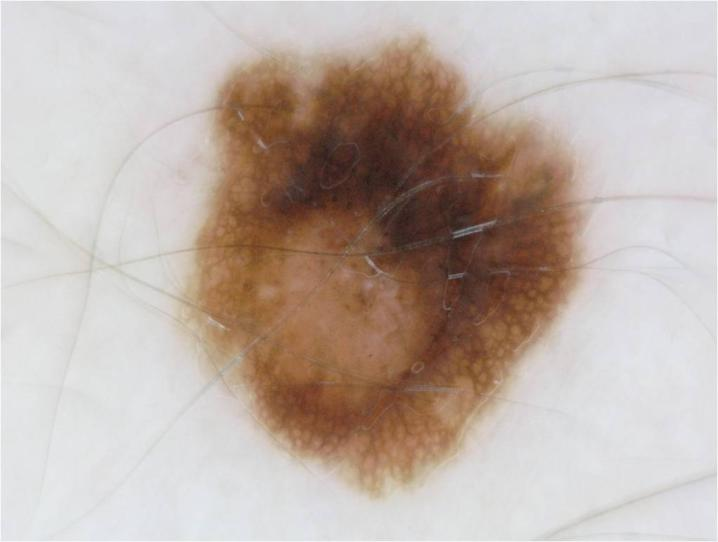
\includegraphics[width=\textwidth]{./pics/augmentations/original.jpg}
		\caption{Original}
		\label{subfig:aug_original}
	\end{subfigure}
	\begin{subfigure}{0.24\linewidth}
		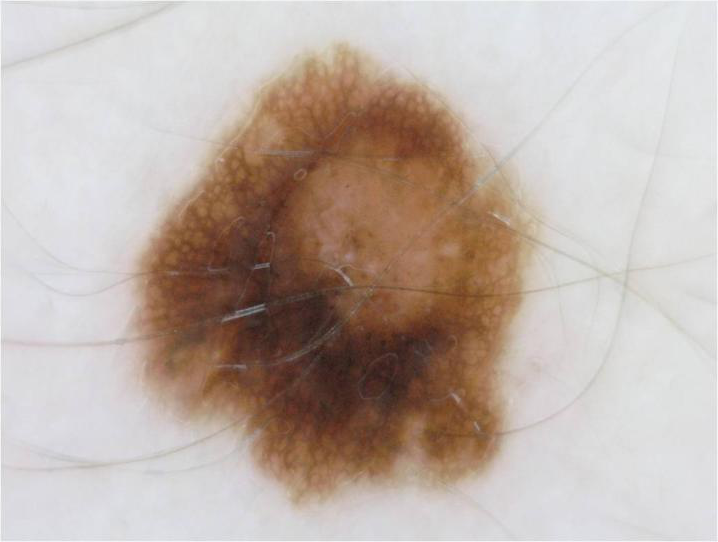
\includegraphics[width=\textwidth]{./pics/augmentations/rotation.png}
		\caption{Rotation}
		\label{subfig:aug_rot}
	\end{subfigure}
	\begin{subfigure}{0.24\linewidth}
		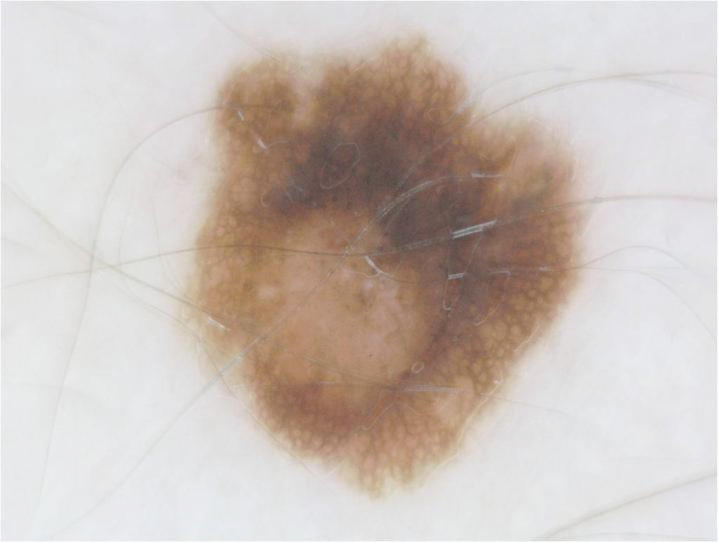
\includegraphics[width=\textwidth]{./pics/augmentations/brightness.png}
		\caption{Helligkeit}
		\label{subfig:aug_bright}
	\end{subfigure}
	\begin{subfigure}{0.24\linewidth}
		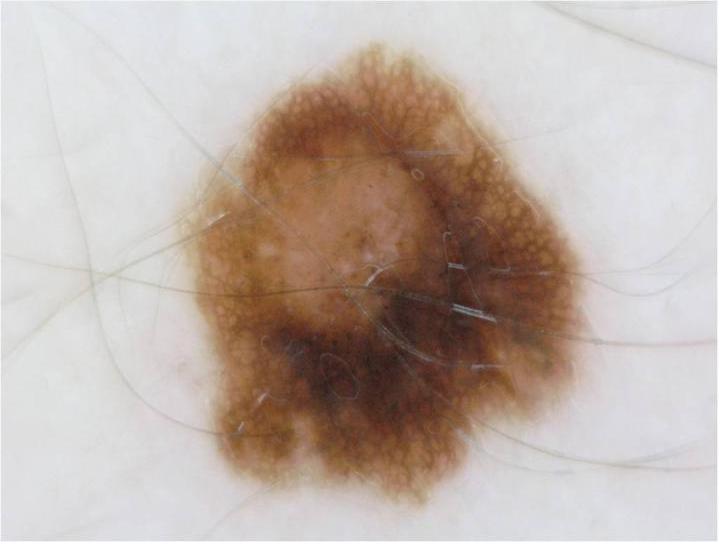
\includegraphics[width=\textwidth]{./pics/augmentations/vertical_flip.png}
		\caption{Vertikale Spiegelung}
		\label{subfig:aug_v_flip}
	\end{subfigure}
	\begin{subfigure}[t]{0.24\linewidth}
		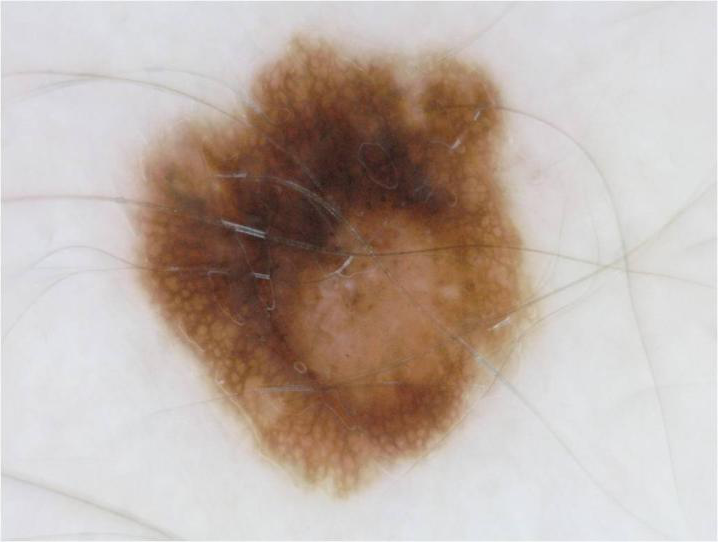
\includegraphics[width=\textwidth]{./pics/augmentations/horizontal_flip.png}
		\caption{Horizontale Spiegelung}
		\label{subfig:aug_h_flip}
	\end{subfigure}
	\begin{subfigure}[t]{0.24\linewidth}
		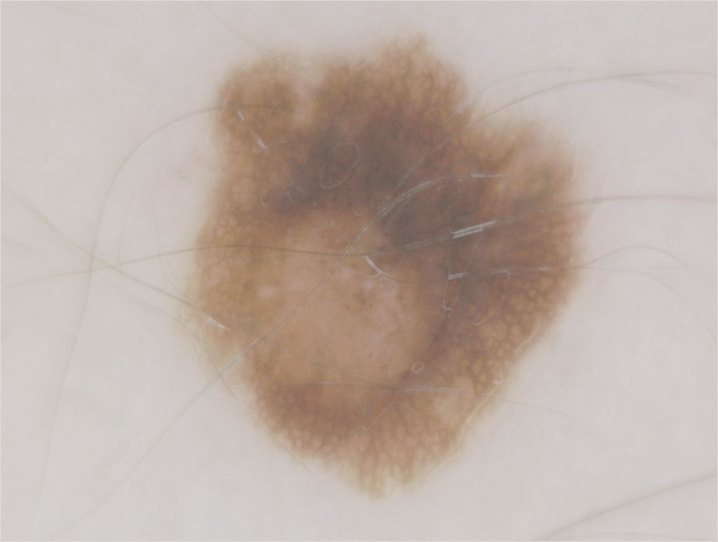
\includegraphics[width=\textwidth]{./pics/augmentations/contrast.png}
		\caption{Kontrast}
		\label{subfig:aug_contrast}
	\end{subfigure}
	\begin{subfigure}[t]{0.24\linewidth}
		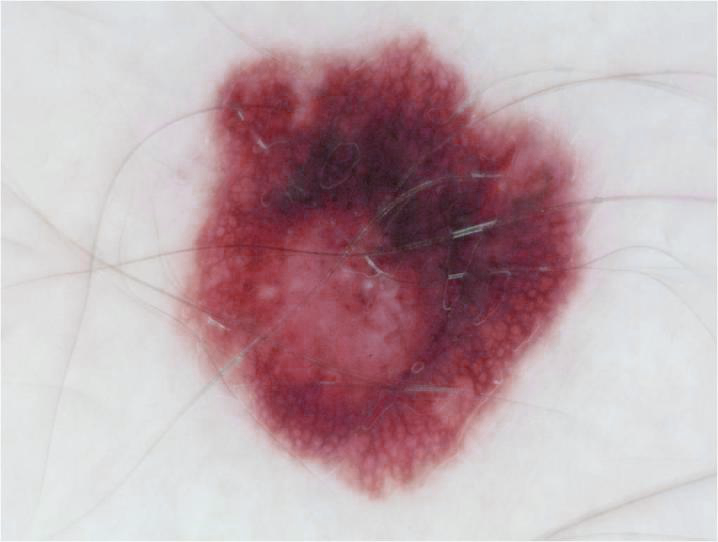
\includegraphics[width=\textwidth]{./pics/augmentations/hue.png}
		\caption{Hue}
		\label{subfig:aug_hue}
	\end{subfigure}
	\begin{subfigure}[t]{0.24\linewidth}
		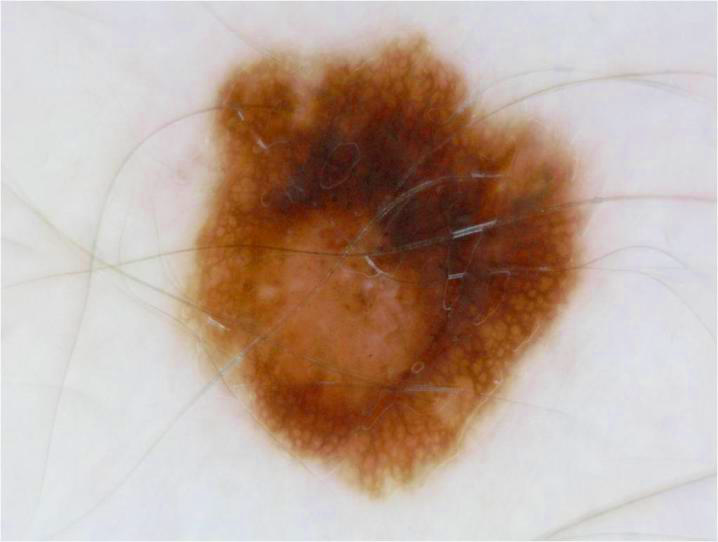
\includegraphics[width=\textwidth]{./pics/augmentations/saturation.png}
		\caption{Sättigung}
		\label{subfig:aug_sat}
	\end{subfigure}
	\caption{Augmentierungsmethoden angewendet auf das orginale Bild (Abbildung \ref{subfig:aug_original})}
\end{figure}


\begin{enumerate}
    \item \textbf{Rotation} (Abbildung \ref{subfig:aug_rot}): Bei dieser Transformation werden die Bilder je um 0$^{\circ}$, 90$^{\circ}$, 180$^{\circ}$ oder 270$^{\circ}$ gedreht. Diese Augmentierung soll das Netz invariant gegenüber Rotation machen. Dies ist wichtig, da die Orientierung der aufgenommenen Bilder willkürlich ist.
    
    \item \textbf{Helligkeit} (Abbildung \ref{subfig:aug_bright}):  Die Helligkeit der Bilder wird hier um einen zufälligen Wert erhöht oder erniedrigt. So soll dem Netz eine gewisse Invarianz gegenüber verschiedenen Lichtbedingungen an trainiert werden.
    
    \item \textbf{Vertikales Spiegeln} (Abbildung \ref{subfig:aug_v_flip}): Hier werden die Bilder vertikal gespiegelt. Hierbei wird die Charakteristik der Läsion nicht verändert, jedoch werden so weitere Trainingsbilder erzeugt. 
    
    \item \textbf{Horizontales Spiegeln} (Abbildung \ref{subfig:aug_h_flip}):  Hier werden die Bilder horizontal gespiegelt. Hierbei wird die Charakteristik der Läsion nicht verändert, jedoch werden so weitere Trainingsbilder erzeugt.
    
    \item \textbf{Kontrast} (Abbildung \ref{subfig:aug_contrast}):  Analog zur Helligkeitsaugmentierung wird hier der Kontrast um einen zufälligen Wert erhöht oder erniedrigt. Auch dies soll das Netz invariant gegenüber wechselnden Lichtverhältnissen machen und zudem die Trainings-Menge vergrößern.
    
    \item \textbf{Hue} (Abbildung \ref{subfig:aug_hue}):  Hier wird der Hue-Wert der Bilder zufällig geändert \todo{schöner schreiben!}. 
    
    \item \textbf{Sättigung} (Abbildung \ref{subfig:aug_sat}):  Die Sättignung der Bilder wird zufällig höher oder niedriger gewählt. Auch dies soll gegen abweichende Lichtverhältnisse helfen und die Trianings-Menge vergrößern.
\end{enumerate}

\subsection{Training}



\color{red}
\begin{itemize}
	\item[\checkmark] Python, Tensorflow, Scikit Learn, NumPy
	\item[\checkmark] Skalierung der Bilder
	\item[\checkmark] Augmentierungsmethoden
	\item Trainingsparameter (Anzahl Durchläufe, Lernrate, Loss-Funktionen)
	\item[\checkmark] Evaluationsmethoden: Berechnung des Scores, etc.
	\item Aufteilung des Datensatzes in Training, Test, Validierung
	\item[\checkmark] genaue Erklärung des Shufflings, da Datensatz nicht ausbalanciert
\end{itemize}
\color{black}

\subsection{Analysemethoden}

Für die Bewertung und Optimierung unseres Klassifizierers wurden verschiedene Methoden angewandt. Die Genauigkeit konnte mit unserem Datensatz nur unter großer Skepsis betrachtet werden. Sie berechnet sich durch die Anzahl der richtig vorhergesagten Beispiele geteilt durch die Anzahl aller Beispiele:
	\[\text{Accuracy} = \frac{TP+TN}{TP+TN+FP+FN}\]
Da der in diesem Projekt verwendete Datensatz deutlich mehr negative als positive Beispiele enthält, können unter dieser Berechnung sehr hohe Genauigkeiten auftreten, obwohl eventuell kein positives Beispiel richtig berechnet wurde. Eine weitaus bessere Analyse ist hierbei möglich indem die richtig-positiv und richtig-negativen Beispiele getrennt angeschaut werden. Die Sensitivität, auch richtig-positiv Rate oder Recall genannt entspricht in unserem Fall den Anteil an tatsächlich malignen Hautläsionen, bei denen die Hautläsion auch als maligne erkannt wurde: 
\[\text{Sensitivität} = \frac{TP}{TP+FN}\]
Die Spezifität, auch richtig-negativ Rate genannt, entspricht dem Anteil an tatsächlich benignen Hautläsionen, die auch als benigne erkannt wurden:
\[\text{Spezifität} = \frac{TN}{TN+FP}\]
Die getrennte Betrachtung beider Werte erlaubt es uns direkt zu sehen ob maligne oder benigne Beispiele besser erkannt werden und dementsprechend zu optimieren.

Zusätzlich zogen wir außerdem noch den \textit{Matthews correlation coefficient} in Betracht. Dieser wird als Qualitätsmaßstab in binären maschinellen Lernmethoden verwendet, im Speziellen wenn der Datensatz sehr unausgeglichen ist. 

\[\text{MCC} = \frac{TP*TN - FP*FN}{\sqrt{(TP+FP)*(TP+FN)*(TN+FP)*(TN+FN)}}\]

Im Gegensatz zu den anderen hier verwendeten Methoden liefert der MCC Werte zwischen $-1$ und $1$. Liefert ein Klassifizierer einen MCC von $0$ so ist er nicht besser als der Zufall. Ein MCC von $1$ hingegen steht für eine komplette Übereinstimmung, ein MCC von $-1$ für die komplette Misklassifizierung.

Schließlich verwendeten wir noch den F1- und F2-Score als Qualitätsmaßstäbe. Der F1-Score ist das harmonische Mittel zwischen dem Recall und der Precision, der F2-Score gewichtet den Recall stärker und setzt somit den Schwerpunkt mehr auf die falsch negativen Stichproben, also die malignen Hautläsionen, die als benigne erkannt wurden:
	\[\text{Precision} = \frac{TP}{TP+FP}\]
    \[\text{Recall/Sensitivität} = \frac{TP}{TP+FN}\]
	\[\text{F1-Score} = 2*\frac{\text{precision}*\text{recall}}	{\text{precision}+\text{recall}}\]
   	\[\text{F2-Score} = 5*\frac{\text{precision}*\text{recall}}	{4*\text{precision}+\text{recall}}\]
    
Wir entschieden uns bewusst für eine größere Anzahl von Qualitätsmaßstäben. Da ein Parameter allein nie die Komplexität des Klassifizierers komplett beschreiben kann, sollen die verschiedenen Qualitätsmaßstäbe bei der Evaluierung und der Entscheidung für den für uns geeignetsten Klassifizierer als Gesamtheit betrachtet und verwendet werden. Dies ermöglicht es uns die Klassifizierung gezielt in die von uns gewünschte Richtung zu lenken um zum Beispiel Falsch-Negative Vorhersagen zu minimieren.
